\documentclass[11pt]{article}
\usepackage{graphicx}
\usepackage{amssymb}
\usepackage{amssymb}
\usepackage{latexsym, amsmath, amscd,amsthm}
\usepackage{graphicx}
\usepackage[percent]{overpic}
\usepackage{pdfsync}
\usepackage{units}
\usepackage{epstopdf}
\usepackage{pdfpages}
\usepackage{listings}

\usepackage{paralist}
\usepackage{color}

\usepackage{forest}

\usepackage{float}
\usepackage{wrapfig}
\usepackage{placeins}

\DeclareGraphicsRule{.tif}{png}{.png}{`convert #1 `dirname #1`/`basename #1 .tif`.png}

%\addtolength{\textwidth}{90pt}
%\addtolength{\evensidemargin}{-60pt}
%\addtolength{\oddsidemargin}{-60pt}
%\addtolength{\topmargin}{-100pt}
%\addtolength{\textheight}{2in}

	\addtolength{\oddsidemargin}{-.875in}
	\addtolength{\evensidemargin}{-.875in}
	\addtolength{\textwidth}{1.75in}

	\addtolength{\topmargin}{-1in}
	\addtolength{\textheight}{2in}

%%%%%%%%%%%%%%%%%%%%%%%%%%%%%%%%%%%%%%%%%%%%%%
% For including sections of code

\usepackage{fancyvrb}
\DefineVerbatimEnvironment{code}{Verbatim}{fontsize=\small}


%%%%%%%%%%%%%%%%%%%%%%%%%%%%%%%%%%%%%%%%%%%%%%
%  Begin user defined commands

\newcommand{\map}[1]{\xrightarrow{#1}}

\newcommand{\C}{\mathbb C}
\newcommand{\F}{\mathbb F}
%\newcommand{\H}{\mathbb H}
%\newcommand{\N}{\mathbb N}
\newcommand{\Z}{\mathbb Z}
\newcommand{\Prob}{\mathbb{P}}
\newcommand{\Q}{\mathbb Q}
\newcommand{\R}{\mathbb R}


\newcommand{\zbar}{\overline{\mathbb{Z}}}
\newcommand{\qbar}{\overline{\mathbb{Q}}}

\newcommand{\la}{\langle}
\newcommand{\ra}{\rangle}
\newcommand{\lra}{\longrightarrow}
\newcommand{\hra}{\hookrightarrow}
\newcommand{\bs}{\backslash}

\newcommand{\al}{\alpha}
\newcommand{\be}{\beta}

%%stats commands
\newcommand{\E}{\mathrm{E}}
\newcommand{\Var}{\mathrm{Var}}
\newcommand{\Cov}{\mathrm{Cov}}

%%% Text Commands
\newcommand{\tand}{\text{ and }}
\newcommand{\tfor}{\text{ for }}
\newcommand{\ton}{\text{ on }}
\newcommand{\tin}{\text{ in }}
\newcommand{\tif}{\text{ if }}

\newcommand{\vectornorm}[1]{\left|\left|#1\right|\right|}

\DeclareMathOperator{\Aut}{Aut}
\DeclareMathOperator{\Aff}{Aff}
\DeclareMathOperator{\End}{End}
\DeclareMathOperator{\Hom}{Hom}
\DeclareMathOperator{\im}{im}

\newcommand{\Gam}{\text{ Gamma}}
\newcommand{\Pois}{\text{ Poisson}}
\newcommand{\Beta}{\text{ Beta}}
\newcommand{\Bin }{\text{ Bin}}
\newcommand{\NegBin}{\text{ NegBin}}

%  End user defined commands
%%%%%%%%%%%%%%%%%%%%%%%%%%%%%%%%%%%%%%%%%%%%%%


%%%%%%%%%%%%%%%%%%%%%%%%%%%%%%%%%%%%%%%%%%%%%%
% These establish different environments for stating Theorems, Lemmas, Remarks, etc.

\newtheorem{Thm}{Theorem}
\newtheorem{Prop}[Thm]{Proposition}
\newtheorem{Lem}[Thm]{Lemma}
\newtheorem{Cor}[Thm]{Corollary}

\theoremstyle{definition}
\newtheorem{Def}[Thm]{Definition}

\theoremstyle{remark}
\newtheorem{Rem}[Thm]{Remark}
\newtheorem{Ex}[Thm]{Example}

\theoremstyle{definition}
\newtheorem{Problem}{Problem}

\newenvironment{Solution}{\noindent{\it Solution.}}{\qed}

\tikzset{
Above/.style={
  midway,
  above,
  font=\scriptsize,
  text width=3.8cm,
  align=center,
  },
Below/.style={
  midway,
  below,
  font=\scriptsize,
  text width=3.8cm,
  align=center
  }
}


% End environments 
%%%%%%%%%%%%%%%%%%%%%%%%%%%%%%%%%%%%%%%%%%%%%%%


\begin{document}

\author{Betsy Cowdery}
\title{Bayesian Statistics HW 2}
\date{}
\maketitle

\begin{enumerate}
	\item Discrete sample spaces: suppose there are N cable cars in San Francisco, numbered sequentially from 1 to N. You see a cable car at random; it is numbered 203. You wish to estimate N. (See Goodman, 1952, for a discussion and references to several versions of this problem, and Jeffreys, 1961, Lee, 1989, and Jaynes, 2003, for Bayesian treatments.)
	\begin{enumerate}
		\item Assume your prior distribution on N is geometric with mean 100; that is,
			$$p(N) = (1/100)(99/100)^{N-1}, \tfor N= 1,2,...$$
			What is your posterior distribution for N?
			
				\[ P(X|N) =  \left\{  
					\begin{array}{ll}
						1/N & \tif N \geq 203 \\
						0 & \tif N < 203
					\end{array}
				\right. \]
			
			Then for $N \geq 203$
			
			\begin{align*}
				P(N|X) &\propto P(N)P(X|N)\\
						&= (1/N)(1/100)(99/100)^{N-1} \\
				P(N|X) &\propto \frac{(99/100)^N}{N}\\
				P(N|X)  &= c \frac{(99/100)^N}{N}
			\end{align*}
			 			
		\item What are the posterior mean and standard deviation of N? (Sum the infinite series analytically or approximate them on the computer.)
		
		We know that $$c = \frac{P(N|X)}{(1/N)(99/100)^N}$$
		
		We also know that 
			\begin{align*}
				1 &= \sum_{N=203}^\infty P(N|X) \\
				c &= \frac{1}{\sum_{N=203}^\infty \frac{(99/100)^N}{N}}
			\end{align*}
			
			We can combine these two equations to get:
			 \begin{align*}
				\frac{P(N|X)}{(1/N)(99/100)^N} &= \frac{1}{\sum_{N=203}^\infty \frac{(99/100)^N}{N}}\\
				P(N|X) &= \frac{(99/100)^N}{N} \frac{1}{\sum_{N=203}^\infty \frac{(99/100)^N}{N}} \\
				&\approx \frac{(99/100)^N}{N}\frac{1}{.04658} \\
				c &\approx \frac{1}{.04658} = 21.47
			\end{align*}
		Then 
		\begin{align*}
			E[N|X] &= \sum_{N=203}^\infty (N * P(N|X)) \\
			&= c \sum_{N=203}^\infty (99/100)^N\\
			&= 21.74 \frac{(99/100)^{203}}{1-(99/100)}\\
			&= 279.1\\
			& \\
			Var(N|X) 
			&= \sum_{N=203}^\infty (N-E[N|X])^2 * P(N|X) \\
			&\approx \sum_{N=203}^\infty (203-279.1)^2 * (21.47) \frac{(99/100)^{203}}{203}\\
			&\approx 6336.16\\
			\sigma(N) &\approx \sqrt(6336.16) = 79.6
		\end{align*} 
		
		\item  Choose a reasonable ‘noninformative’ prior distribution for N and give the resulting posterior distribution, mean, and standard deviation for N.
			
			I'm going to recycle some of my answer from problem 3 and use Jeffrey's prior for a geometric distribution:\\
			Given that $\E[X|N] = 1/N$
			\begin{align*}
	I(N) 
	&= -\E \left[ \left. -\frac{1}{N^2}-\frac{X-1}{(1-N)^2} \right| \theta \right]\\
	&= -\frac{1}{N^2}+\frac{\frac{1}{N}-1}{(1-N)^2}\\
	&= \frac{1}{N^2(1-N)}
\end{align*}

Therefore $$P_J(N) = I(N)^{\frac{1}{2}} \propto N^{-1}(1-N)^{-\frac{1}{2}}= \Beta \left(0,\frac{1}{2}\right)$$
This is an improper distribution, but the posterior will be proper for $X\geq1$.
			\begin{align*}
				P(X|N) &=  N^{X-1}(1-N)^{N-X-1}\\
				& \\
				P(N|X) &\propto P(N)P(X|N)\\
						&= (N^{-1}(1-N)^{-\frac{1}{2}})( N^{X-1}(1-N)^{N-X-1}) \\
				 		&=  N^{X-2}(1-N)^{N-X-\frac{3}{2}}\\
				 		&= \Beta (-1,\frac{1}{2})
			\end{align*}
			
					Then 
		\begin{align*}
			E[N|X] &= \sum_{N=0}^{203} (N *  N^{X-2}(1-N)^{N-X-\frac{3}{2}}) \\
			&= \sum_{N=0}^{203} (N^{X-1}(1-N)^{N-X-\frac{1}{2}})
			& \\
			Var(N|X) 
			&= \sum_{N=203}^\infty (N-E[N|X])^2 * P(N|X) \\
			&\approx \sum_{N=203}^\infty (203-279.1)^2 * (21.47) \frac{(99/100)^{203}}{203}\\
			&\approx 6336.16\\
			\sigma(N) &\approx \sqrt(6336.16) = 79.6
		\end{align*}
		
	\end{enumerate}
	
\rule{0.94\textwidth}{0.4pt}

	\item Discrete data: Table 2.2 gives the number of fatal accidents and deaths on scheduled airline flights per year over a ten-year period. We use these data as a numerical example for fitting discrete data models.

	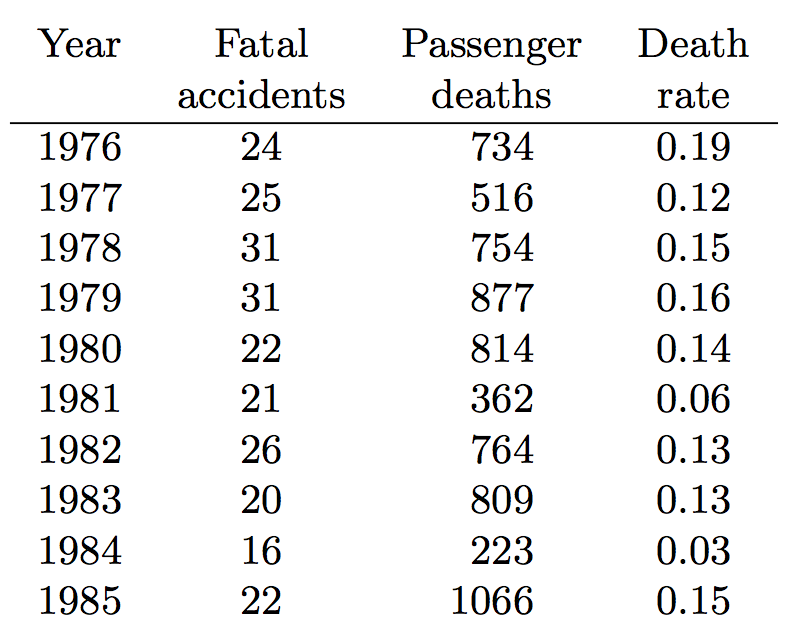
\includegraphics[width = 0.4\textwidth]{Table_22}
	
	Passenger Miles Flown = $\{3.836,4.3,5.027,5.481,6.033,5.877,6.223,7.433,7.106\} \times 10^{11}$
	
\begin{enumerate}
	\item Assume that the numbers of fatal accidents in each year are independent with a Poisson($\theta$) distribution. Set a prior distribution for $\theta$ and determine the posterior 	distribution based on the data from 1976 through 1985. Under this model, give a 95\% predictive interval for the number of fatal accidents in 1986. You can use the normal approximation to the gamma and Poisson or compute using simulation.
	
			$$y_i|\theta \sim \text{Poisson}(\theta)$$
		where \begin{align*}
			y_i &= \text{number of fatal accidents in year } i \in {1,...,10} \\
			\theta &= \text{expected number of accidents per year}
		\end{align*} 
	Then the prior distribution for $\theta$ is $\theta \sim \text{Gamma}(\alpha, \beta) $\\
	And the posterior distribution is $\theta|y \sim \text{Gamma}(\alpha + 10\bar{y}, \beta + 10) $
	
	Because we have $n=10$ we can be comfortable using an informative prior, setting $(\alpha,\beta)=0$ \\
	Thus $\theta|y = \Gam(238,10)$ with 95\% predictive interval 
	
	If $\tilde y$ is the number of fatal accidents in 1986, then $\tilde y \sim \Pois(\theta)$ with a computed 95\% predictive interval of $[15,35]$\\
	
	\item Assume that the numbers of fatal accidents in each year follow independent Poisson distributions with a constant rate and an exposure in each year proportional to the number of passenger miles flown. Set a prior distribution for $\theta$ and determine the posterior distribution based on the data for 1976–1985. (Estimate the number of passenger miles flown in each year by dividing the appropriate columns of Table 2.2 and ignoring round-off errors.) Give a 95\% predictive interval for the number of fatal accidents in 1986 under the assumption that $8 \times 10^{11}$ passenger miles are flown that year.\\
		
		Let \\
		$m_i$ be the number of passenger miles flown in year $i$\\
		$\theta$ be expected accident rate per passenger mile\\
		If we assume an informative prior $\theta \sim \Gam(0,0)$\\
		Then 
		
		\begin{align*}
		y_i | m_i \theta &\sim \Pois (m_i\theta) \\
		y| m \theta &\sim \Pois (m\theta) \\
		y|\theta &\sim \Gam (10\bar y, 10 \bar m) \\
		&= \Gam (238, 5.716 \times 10^{12} )
		\end{align*}
		
		Then the predictive distribution $\tilde y \sim \Pois (\tilde m\theta)$\\ and the calculated 95\% predictive interval is $[22, 46]$ \\
		 
	\item Repeat (a) above, replacing ‘fatal accidents’ with ‘passenger deaths.’\\
		
	Let $d_i$ be the number of passenger deaths in year $i \in {1,...,10}$\\ $\theta$ be the expected number of accidents per year
	
	Assume an uninformative prior $\theta \sim \text{Gamma}(0,0)$
	
	And the posterior distribution 
	\begin{align*}
		\theta|y & \sim \Gam( 10\bar{d}, 10)\\
		&= \Gam(6919, 10)
	\end{align*} 

	Predictive distribution $\tilde d \sim \Pois(\theta)$\\
	and the calculated 95\% predictive interval is $[638, 749]$\\
	
	\item Repeat (b) above, replacing ‘fatal accidents’ with ‘passenger deaths.’\\

		Let \\
		$m_i$ be the number of passenger miles flown in year $i$\\
		$\theta$ be expected accident rate per passenger mile\\
		If we assume an informative prior $\theta \sim \Gam(0,0)$\\
		Then 		\begin{align*}
		d_i | m_i \theta &\sim \Pois (m_i\theta) \\
		d| m \theta &\sim \Pois (m\theta) \\
		d|\theta &\sim \Gam (10\bar d, 10 \bar m) 
		\end{align*}
		
		
		Then the predictive distribution $\tilde d \sim \Pois (\tilde m\theta) $\\
		and the calculated 95\% predictive interval is $[905, 1032]$ \\

	\item In which of the cases (a)-(d) above does the Poisson model seem more or less reasonable? Why? Discuss based on general principles, without specific reference to the numbers in Table 2.2.\\
		
		In general I think that a model in which number of deaths are dependent on the number of miles flown, since intuitively if more people are flying, then the probability of someone getting in an accident is larger and vice versa. This leaves us with (b) and (d). Furthermore, while fatal accidents are independent, passenger deaths are not - since if a passenger dies it most likely is the result of a fatal accident in which other passengers may have died. This narrows down the choices to case (b) as the most reasonable of the four models. 
		
\end{enumerate}

\rule{0.94\textwidth}{0.4pt}
\item Suppose that you keep trying Bernoulli experiments with probability of success $\theta$ until you have $r$ failures, and you observe $X | \theta \sim NegBin(r, \theta)$ successes.
	

	$r > 0 $ is the number of failures until the experiment is stopped (success)\\
	$x \geq r $ is the number of successes (failure)\\
	$0 < \theta < 1$ is the probability of success
	\begin{align*}
		X|\theta &\sim NegBin(r, \theta)\\
		X|\theta &\propto \left( \begin{array}{c} x + r -1 \\ x \end{array} \right)\theta^r (1-\theta)^x
	\end{align*}
	
	
	\begin{enumerate}
		\item Find the conjugate prior of $\theta$ for this likelihood. How does it compare to the conjugate prior for a binomial likelihood?

			Suppose we define $\theta \sim \text{Beta}(\alpha,\beta)$\\
			Then 
\begin{align*}
	P(\theta|X) &\propto \left( \begin{array}{c} x + r -1 \\ x \end{array} \right)\theta^r (1-\theta)^x  \frac{\theta^{\alpha-1}(1-\theta)^{\beta -1}}{\text{Beta}(\alpha,\beta)}\\
	&\propto \theta^{\alpha+r-1} (1-\theta)^{\beta+x-1}
\end{align*}
And thus $\theta|X \sim \Beta (\alpha+r , \beta+x)$

We can generalize this by realizing that the negative binomial and the binomial have likelihood functions of the form $\theta|X \propto c \theta^a (1-\theta)^b $ where $c$ is a normalizing constant. 
Then \begin{align*}
	P(\theta|X) &\propto c\theta^a (1-\theta)^b  \frac{\theta^{\alpha-1}(1-\theta)^{\beta -1}}{\text{Beta}(\alpha,\beta)}\\
	&\propto \theta^{\alpha+a-1} (1-\theta)^{\beta+b-1}
\end{align*}
And once again $\theta|X \sim \Beta (\alpha+a , \beta+b)$. \\
Thus the conjugate prior will be the same in both cases.  

		\item Find Jeffrey’s prior for this likelihood. Is it proper? How does it compare to Jeffrey’s prior for a binomial likelihood?
			
			We know that the Fisher information for $\theta$ is: 
			$$I(\theta) = -\E \left[ \left. \frac{d^2 log P(X|\theta)}{d\theta^2} \right| \theta \right]$$ 		
Again, using the generalized likelihood function for the binomial and negative binomial cases,
\begin{align*}
	I(\theta) &= -\E \left[ \left.\frac{d^2}{d\theta^2}\log (c (1-\theta)^a \theta^b)  \right| \theta \right]\\
	 &= -\E \left[ \left.\frac{-((\theta-1)^2 a+\theta^2 b)}{(\theta-1)^2 \theta^2}\right| \theta \right]\\
	 &= -\E \left[ \left. -\frac{a}{\theta^2}-\frac{b}{(1-\theta)^2} \right| \theta \right]\\
\end{align*}		
		
Then Jeffrey's prior \\
for Binomial: \\
$ a = x \\ b = n-x $

Since $\E[X] = n\theta$
\begin{align*}
	I(\theta) 
	&= -\E \left[ \left. -\frac{x}{\theta^2}-\frac{n-x}{(1-\theta)^2} \right| \theta \right]\\
	&= -\E \left[ \left. -\frac{n\theta}{\theta^2}-\frac{n-n\theta}{(1-\theta)^2} \right| \theta \right]\\
	&= \frac{n\theta}{\theta^2}+\frac{n-n\theta}{(1-\theta)^2}\\
	&= \frac{n}{\theta(1-\theta)}
\end{align*}

Therefore $$P_J(\theta) = I(\theta)^{\frac{1}{2}} \propto \theta^{-\frac{1}{2}}(1-\theta)^{-\frac{1}{2}}= \Beta \left(\frac{1}{2},\frac{1}{2}\right)$$
This is a proper distribution. 

for Negative Binomial:\\ 
$ a = x \\ b = r $

Since $\E[X] = \frac{r\theta}{1-\theta}$
\begin{align*}
	I(\theta) 
	&= -\E \left[ \left. -\frac{x}{\theta^2}-\frac{r}{(1-\theta)^2} \right| \theta \right]\\
	&= -\E \left[ \left. -\frac{r\theta}{1-\theta}*\frac{1}{\theta^2}-\frac{r}{(1-\theta)^2} \right| \theta \right]\\
	&= \frac{r\theta}{(1-\theta)\theta^2}+\frac{r}{(1-\theta)^2}\\
	&= \frac{r}{\theta^2(1-\theta)}
\end{align*}
Therefore $$P_J(\theta) = I(\theta)^{\frac{1}{2}} \propto \theta^{-1}(1-\theta)^{-\frac{1}{2}} = \Beta \left( 0,\frac{1}{2} \right)$$
	This is a uniform distribution and therefore not proper. 
	\end{enumerate}
\end{enumerate}































\end{document}